\cleardoublepage % memastikan bab baru dimulai di halaman ganjil (kanan)
\chapter{DASAR TEORI}
\label{chap:dasar-teori}

\section{Data Multimedia dan Representasinya}
\label{data_mm}

Keberadaan data merupakan suatu hal yang krusial dalam proses pengembangan platform ADADeH. Data yang menjadi fondasi utama pengembangan ADADeH merupakan data multimedia. Pengembangan platform ini setidaknya mencakup dua data multimedia: (1) audio sebagai data utama dan (2) citra spektrogram frekuensi audio terhadap waktu yang menjadi masukan model. Data-data tersebut berkontribusi dalam mengklasifikasi audio asli dan audio buatan AI generatif (\textit{deepfake audio}).

\subsection{Data Audio}
\label{data_audio}

Menurut \textcite{winer2025audio}, audio pada dasarnya adalah gelombang suara berbentuk pola kompresi dan ekspansi yang merambat melalui medium tertentu pada rentang frekuensi yang dapat didengar manusia. Rentang tersebut ada pada kisaran 20~Hz--20~kHz \autocite{wikipedia2026hearingrange}. Medium rambat gelombang suara umumnya adalah udara. Pada produksi musik atau audio digital, apabila gelombang tersebut ditangkap dari udara oleh media elektronik seperti mikrofon, suara dapat direpresentasikan sebagai sinyal listrik yang dialirkan melalui kabel atau sirkuit.

Dalam TPdK ini, audio berperan sebagai data primer yang diolah dan nantinya dilatih model. Pemanfaatan audio sebagai data perlu memerhatikan beberapa hal, yaitu:
\begin{enumerate}[(a).]
  \item \textit{Sampling rate} (\textit{sr}). Menurut \textcite{shannon1949}, sinyal yang tidak memuat frekuensi di atas $F$ dapat direkonstruksi apabila dicuplik minimal $2F$ kali per detik. Audio diseragamkan pada \textit{sr} yang sama sebelum diubah ke spektrogram.
  \item Format dan \textit{codec}. \textit{Dataset} yang digunakan menyimpan rekaman dalam format FLAC (\textit{Free Lossless Audio Codec}), yaitu format kompresi audio secara \textit{lossless} sehingga sinyal dekode identik dengan sinyal asli \autocite{rfc9639flac}. Hal ini berbeda dengan MP3 yang menggunakan kompresi \textit{lossy} dan membuang sebagian informasi sinyal \autocite{brandenburg1999mp3}.
  \item Jumlah kanal dan durasi. Audio perlu diseragamkan menjadi satu kanal (mono) berdurasi tetap, agar menghasilkan spektrogram berdimensi seragam.
\end{enumerate}

\subsection{Data Citra Spektrogram}
\label{data_spektrogram}

Spektrogram adalah citra dua dimensi yang memuat grafik representasi gelombang suara (\textit{waveform}) terhadap waktu. Umumnya, grafik ini menempatkan frekuensi suara pada sumbu-Y dan waktu pada sumbu-X \autocite{app16020572}. Spektrogram direpresentasikan sebagai matriks vektor frekuensi bertumpuk yang tiap tumpukannya mewakili magnitudo frekuensi pada bingkai waktu singkat (\textit{analysis frame}). Pembentukkan spektrogram diilustrasikan pada Gambar \ref{fig:form_spectrogram}.

\begin{figure}[h]
  \centering
  \caption{Proses Pembentukkan Spektrogram \autocite{app16020572}} 
	\label{fig:form_spectrogram}
    	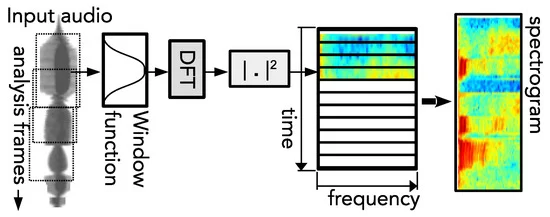
\includegraphics[width=0.7\textwidth]{images/form_of_spec.png}
\end{figure}

Setiap vektor magnitudo frekuensi merupakan hasil dari transformasi ortogonal frekuensi suara terhadap waktu seperti \textit{Discrete Fourier Transform} (DFT), \textit{Fast Fourier Transform} (FFT), \textit{Discrete Cosine Transform} (DCT), dan sebagainya \autocite{mcloughlin2016speech}. Proses dilanjutkan dengan penjedelaan tiap potongan audio melalui fungsi jendela (\textit{window function}) untuk mencegah kebocoran spektral (\textit{spectral leakage}) dan efek tepi (\textit{edge effect}) \autocite{gibbs1899fourier}. Hal ini dilakukan karena fungsi jendela biasanya meredup hingga nol atau mendekati nol di tepi setiap bingkai.

Salah satu bentuk pengembangan spektrogram adalah \textit{mel-spectrogram}. Bentuk tersebut digunakan pada TPdK ini yang akan lebih lanjut pada Subsubbab \ref{melspektrogram}. Selain itu beberapa perlakuan khusus yang harus diterapkan pada grafik spektrogram sebelum dilatih oleh model secara umum akan dijelaskan pada Subsubbab \ref{proc_spektrogram}

\subsubsection{\textit{Mel-Spectrogram}}
\label{melspektrogram}

Representasi frekuensi terhadap waktu yang dipetakan pada skala Mel disebut \textit{mel-spectrogram}. Skala ini pertama kali digagas oleh \textcite{stevens1937mel} dengan menerapkan pemanfaatan data kenyaringan setara (\textit{equal-loudness}) manusia untuk pemetaan frekuensi (Hz) ke skala non-linear sesuai dengan persepsi manusia. Pada skala ini, selisih nilai yang sama berkorespondensi dengan selisih tinggi nada yang terdengar sama bagi pendengar, sehingga resolusinya lebih rapat pada frekuensi rendah dan lebih renggang pada frekuensi tinggi. Secara umum, pemetaan dari frekuensi linear (${f_{Hz}}$) ke frekuensi mel (${f_{mel}}$) mengikuti formula komputasi di bawah:

\begin{align}
  f_{mel} = 2595 \log_{10}\left(1 + \frac{f_{Hz}}{700}\right)
  \label{eq:hz_to_mel}
\end{align}
\eqcaption{Persamaan Pemetaan Frekuensi Linear ke Mel}

Persamaan \ref{eq:hz_to_mel} di atas menunjukkan bahwa pada ${f_{Hz} \le 700}$, hubungan antara ${f_{Hz}}$ dan ${f_{mel}}$ akan mendekati linear. Sedangkan pada ${f_{Hz} > 700}$ nilai mel akan bertambah semakin lambat secara logaritmik. Frekuensi Mel yang terhitung akan menjadi tumpukkan vektor seperti halnya pada spektrogram linear. Berdasarkan keserupaan tersebut, luaran yang dihasilkan adalah suatu grafik yang disebut \textit{mel-spectrogram}. 

Karena proses pembentukannya melibatkan skala Mel yang dikembangkan dari eksperimen persepsi pendengaran manusia, \textit{mel-spectrogram} terbukti efektif untuk berbagai tugas analisis ucapan (\textit{speech analysis}). Keefektifan tersebut berpotensi mendukung pengembangan platform ADADeH yang fokus utamanya adalah menganalisis baik ucapan asli manusia maupun ucapan sintesis buatan AI. Selain itu, model pembelajaran mendalam atau DL (\textit{Deep Learning}) cenderung memiliki kemampuan lebih baik dalam memproses data citra dibanding data audio mentah. Model DL seperti CNN (\textit{Convolutional Neural Network}) merupakan salah satu model dengan kemampuan tersebut. Model ini akan dijabarkan secara rinci pada Subbab \ref{other_tech}.

\subsubsection{Pemrosesan Spektrogram}
\label{proc_spektrogram}

Meskipun spektrogram umumnya tersaji dalam bentuk citra dua dimensi yang diproses oleh model DL, pada dasarnya spektrogram adalah grafik. Hal ini menjadi kurang tepat jika pemrosesan datanya diserupakan dengan data citra lainnya. \autocite{app16020572} memaparkan bahwa ada beberapa penyesuian yang perlu dilakukan pada citra spektrogram. Beberapa perlakuan tersebut tersaji pada rincian di bawah:
\begin{enumerate}
  \item Pemilihan Warna (Berwarna/RGB atau \textit{Greyscale})
  \begin{itemize}
    \item Spektrogram pada dasarnya \textit{greyscale} dengan nilai piksel 0 (putih)--1 (hitam). Pemberian warna pada spektrogram bisa saja dilakukan tapi hanya terbatas untuk keperluan visualisasi.
    \item Memasukkan spektrogram berwarna pada model DL (seperti CNN) tidak menyebabkan kegagalan pembelajaran model.
    \item Memasukkan spektrogram RGB pada model DL berimbas pada tingginya kompleksitas masukan (yaitu tiga kali lipat daripada \textit{greyscale}). Hal ini disebabkan bahwa citra RGB memiliki 3 kanal atau \textit{channel} warna, sedangkan greyscale hanya terdiri atas 1 kanal warna.
  \end{itemize}
  \item Invariansi Translasi dan Skala
  \begin{itemize}
    \item Pada citra, objek yang digeser tetaplah objek yang sama. Hal ini berbeda dengan spektrogram yang memuat grafik frekuensi suara--waktu.
    \item Pada spektrogram, pergeseran sepanjang waktu (sumbu-X) tidak mengubah isi suara, tetapi pergeseran sepanjang frekuensi (sumbu-Y) bisa membuatnya terdengar seperti suara lain. Informasi yang terkandung pada sumbu X dan Y punya makna yang berbeda.
    \item Perubahan skala secara horizontal berimbas pada durasi (cepat atau lambatnya suara). Perubahan skala secara vertikal berimbas pada rentang frekuensi suara (tinggi atau rendahnya nada).
    \item Hal penting lainnya adalah mempertahankan konsistensi parameter spektrogram pada tahap prapemrosesan dan pelatihan model. Hal ini bertujuan agar skala spektrogram yang diterima model sama sehingga model tidak salah membaca data.
  \end{itemize}
  \item Fitur Lokal
  \begin{itemize}
    \item Korelasi lokal dan global pada audio berbeda sifatnya dengan pada citra.
    \item Pola serupa pada rentang 0--50~Hz dan 16--18~kHz belum tentu bermakna, sedangkan pada citra bagian tekstur yang serupa (misalnya rumput) saling berkaitan dan penting untuk mendukung tugas klasifikasi.
    \item Korelasi lokal sepanjang waktu lebih mirip selisih antar-frame video daripada titik yang berdekatan pada citra.
  \end{itemize}
\end{enumerate}

\section{Sistem Multimedia}
\label{sist_mulmed}

Menurut \textcite{bandung2025inovasi}, multimedia setidaknya mengacu pada penggunaan berbagai jenis media yang meliputi teks, gambar, grafik, video, audio, animasi dan sebagainya, dalam satu lingkungan terintegrasi. Lingkungan tersebut harus memiliki kapabilitas untuk memproses, menyimpan, dan mengirim media melalui jaringan komunikasi data. Lebih lanjut, terminologi sistem multimedia merujuk pada kombinasi media-media tersebut yang tersalur pada beragam aplikasi \autocite{furht1994overview}. 

Selain itu, \textcite{furht1994overview} juga menuturkan bahwa dalam praktiknya, sistem multimedia dapat menyimpan informasi audio dan video untuk dipakai kemudian, atau mentransmisikannya secara langsung (\textit{live-stream}) secara \textit{real-time}. Hal ini menyebabkan kompleksitasnya bertumpu pada seluruh komponen sistem komputer, mulai dari daya pemrosesan, penyimpanan, hingga jaringan digunakan. Dalam penerapannya pada sistem komputer, sistem multimedia kian berkembang pemanfaatannya seiring dengan berkembangnya teknologi seperti pembelajaran mendalam atau \textit{deep learning} (DL) \autocite{li2021fundamentals}. Hal inilah yang diimplementasikan pada ADADeH.

ADADeH memposisikan sistem multimedia melalui alur pengolahan data audio. Alur ini setidaknya meliputi akuisisi, prapemrosesan, analisis model, dan penyajian model. Pada tahap akuisisi, data audio diterima dalam format FLAC (Subbab \ref{data_audio}) pada cuplikan tertentu (2,5--12,5 detik) yang konsisten. Selanjutnya data diolah pada tahap prapemrosesan dengan didekode ke plot gelombang audio (\textit{waveform}), diseragamkan menjadi satu kanal dengan \textit{sampling rate} dan durasi tetap, diurai dalam beberapa potongan (\textit{chunks}), kemudian ditransformasi melalui \textit{Short-Time Fourier transform} (STFT) dan \textit{filter bank} mel, dikonversi ke skala logaritmik (dB), serta dinormalisasi menggunakan statistik data latih untuk menghasilkan \textit{mel-spectrogram}. Selanjutnya \textit{mel-spectrogram} akan dilatih pada model DL untuk tugas klasifikasi.

Pada tahap analisis model, \textit{mel-spectrogram} $\mathbf{X} \in \mathbb{R}^{M \times T}$, dengan $M$ jumlah \textit{mel bin} dan $T$ jumlah \textit{frame} waktu, diperlakukan sebagai citra satu kanal dan diproses oleh \textit{convolutional neural network} (CNN). Lapisan konvolusi mengekstraksi fitur lokal dengan menggeser filter berukuran $k_h \times k_w$ pada spektrogram, diikuti fungsi aktivasi ReLU (Persamaan~\ref{eq:conv}). Fitur yang dihasilkan diringkas oleh lapisan \textit{pooling} dan diteruskan ke lapisan \textit{fully connected} yang menghasilkan satu nilai skalar $z$ (\textit{logit}).

\begin{align}
  Z_k[i,j] = \max\left(0,\; b_k + \sum_{c=1}^{C_{\mathrm{in}}} \sum_{m=0}^{k_h-1} \sum_{n=0}^{k_w-1} W_k[c,m,n]\, X_c[i+m,\, j+n]\right)
  \label{eq:conv}
\end{align}
\eqcaption{Persamaan Lapisan Konvolusi dengan Aktivasi ReLU}

Nilai tersebut dikonversi menjadi probabilitas audio \textit{deepfake} $p$ menggunakan fungsi sigmoid (Persamaan~\ref{eq:sigmoid}).

\begin{align}
  p = \sigma(z) = \frac{1}{1 + e^{-z}}
  \label{eq:sigmoid}
\end{align}
\eqcaption{Persamaan Fungsi Sigmoid}

Kemudian label prediksi $\hat{y}$ ditentukan dengan membandingkan $p$ terhadap ambang $\tau$ (Persamaan~\ref{eq:threshold}).

\begin{align}
  \hat{y} =
  \begin{cases}
    1 & \text{jika } p \geq \tau \\
    0 & \text{jika } p < \tau
  \end{cases}
  \label{eq:threshold}
\end{align}
\eqcaption{Persamaan Penentuan Label Prediksi}

Selama pelatihan, parameter model dioptimasi dengan meminimalkan \textit{binary cross-entropy} (Persamaan~\ref{eq:bce}).

\begin{align}
  \mathcal{L} = -\frac{1}{N} \sum_{i=1}^{N} \left[ y_i \log p_i + (1 - y_i) \log (1 - p_i) \right]
  \label{eq:bce}
\end{align}
\eqcaption{Persamaan \textit{Binary Cross-Entropy}}

Pada tahap penyajian hasil, ADADeH menampilkan label prediksi (asli atau \textit{deepfake}) beserta skor keyakinan $c = \max(p,\, 1-p)$ kepada pengguna.

\section{Perangkat Keras dan Perangkat Lunak}
\label{soft_hard_ware}

Alur pengolahan audio pada Subbab \ref{sist_mulmed} membutuhkan perangkat untuk menjalankannya. Berbeda dengan sistem multimedia yang bergantung pada sensor atau mikrokontroler, ADADeH seluruhnya berjalan di atas komputer umum dan layanan komputasi awan (\textit{cloud}). Oleh karena itu, subbab ini hanya membahas perangkat yang dipakai selama pengembangan purwarupa, yaitu perangkat keras pada Subbab \ref{hardware} dan perangkat lunak pada Subbab \ref{software}.

\subsection{Perangkat Keras}
\label{hardware}

Perangkat keras pada TPdK ini dibagi berdasarkan perannya, yaitu perangkat untuk melatih model, perangkat untuk mengembangkan dan menjalankan purwarupa, serta perangkat di sisi pengguna.

\subsubsection{Perangkat Pelatihan Model}
\label{hw_training}

Pelatihan model merupakan tahap yang paling berat secara komputasi. Pada tahap ini, operasi konvolusi pada Persamaan \ref{eq:conv} dihitung berulang kali untuk seluruh \textit{mel-spectrogram} pada data latih, dan diulang lagi di setiap \textit{epoch} (satu putaran penuh atas data latih). Jika hanya mengandalkan CPU (\textit{Central Processing Unit}), proses tersebut dapat memakan waktu yang sangat lama. Hal inilah yang membuat GPU (\textit{Graphics Processing Unit}) dibutuhkan.

GPU awalnya dirancang untuk mengolah grafis, tetapi memiliki ribuan inti kecil yang dapat mengerjakan banyak perhitungan sederhana secara bersamaan. Sifat ini cocok dengan operasi konvolusi, yang pada dasarnya adalah perkalian dan penjumlahan matriks dalam jumlah besar.

Pelatihan model ADADeH dilakukan pada Kaggle Notebook, yaitu layanan komputasi awan yang menyediakan GPU secara gratis dengan kuota waktu tertentu tiap pekan \autocite{kaggle2026notebooks}. Layanan ini dipilih karena \textit{dataset} yang digunakan juga tersedia di Kaggle, sehingga data dapat langsung dipasang ke \textit{notebook} tanpa perlu diunduh dan diunggah ulang. Spesifikasi perangkat yang disediakan tersaji pada Tabel \ref{tab:spek_training}. Peran tiap komponennya adalah sebagai berikut:
\begin{enumerate}[(a).]
  \item GPU dan VRAM (\textit{Video Random Access Memory}). GPU mengerjakan perhitungan model, sedangkan VRAM adalah memori milik GPU yang menampung parameter model beserta sekumpulan data (\textit{batch}) yang sedang diproses. Kapasitas VRAM membatasi banyaknya \textit{mel-spectrogram} yang dapat diproses dalam satu \textit{batch}.
  \item CPU. Walaupun perhitungan model dikerjakan GPU, CPU tetap berperan dalam mendekode berkas FLAC, membentuk \textit{mel-spectrogram}, dan menyusun \textit{batch} sebelum dikirim ke GPU.
  \item RAM (\textit{Random Access Memory}). RAM menampung data yang sedang diolah CPU. Jika kapasitasnya kurang, proses pelatihan dapat terhenti di tengah jalan.
  \item Media penyimpanan. Media ini menyimpan \textit{dataset} audio dan berkas model hasil pelatihan yang nantinya dimuat kembali oleh purwarupa.
\end{enumerate}

\begin{table}[t]
  \centering
  \caption{Spesifikasi perangkat pelatihan model pada Kaggle Notebook}
  \label{tab:spek_training}
  \begin{tabularx}{0.8\textwidth}{| l | X |}
    \hline
    \textbf{Komponen} & \textbf{Spesifikasi} \\
    \hline
    GPU   & (isi, misalnya NVIDIA Tesla T4) \\
    VRAM  & (isi) GB \\
    CPU   & (isi jumlah inti dan tipenya) \\
    RAM   & (isi) GB \\
    Penyimpanan & (isi) GB \\
    \hline
  \end{tabularx}
\end{table}

\subsubsection{Perangkat Pengembangan dan Pengujian}
\label{hw_dev}

Laptop digunakan untuk menulis kode, menyusun laporan, dan menjalankan purwarupa ADADeH. Berbeda dengan pelatihan, proses prediksi (\textit{inference}) jauh lebih ringan. Model cukup menghitung keluaran satu kali untuk tiap potongan audio tanpa perlu memperbarui parameternya. Oleh karena itu, purwarupa dapat dijalankan pada laptop tanpa GPU khusus. Spesifikasi laptop yang digunakan tersaji pada Tabel \ref{tab:spek_laptop}.

\begin{table}[t]
  \centering
  \caption{Spesifikasi laptop pengembangan dan pengujian}
  \label{tab:spek_laptop}
  \begin{tabularx}{0.8\textwidth}{| l | X |}
    \hline
    \textbf{Komponen} & \textbf{Spesifikasi} \\
    \hline
    Merek dan tipe  & (isi) \\
    Prosesor        & (isi) \\
    RAM             & (isi) GB \\
    Penyimpanan     & (isi, misalnya SSD 512 GB) \\
    Kartu grafis    & (isi) \\
    Sistem operasi  & (isi) \\
    \hline
  \end{tabularx}
\end{table}

\subsubsection{Perangkat Pengguna}
\label{hw_user}

Dari sisi pengguna, ADADeH tidak membutuhkan perangkat khusus. Pengguna cukup memiliki perangkat yang dapat menyimpan dan mengunggah rekaman audio, misalnya ponsel pintar atau laptop. Meskipun begitu, ada dua komponen pada perangkat perekam yang berpengaruh langsung pada kualitas rekaman, yaitu:
\begin{enumerate}[(a).]
  \item Mikrofon. Seperti dijelaskan pada Subbab \ref{data_audio}, mikrofon menangkap gelombang suara dari udara dan mengubahnya menjadi sinyal listrik. Mikrofon bawaan ponsel sudah memadai untuk merekam ucapan, tetapi suara bising di sekitar perekam akan ikut terekam.
  \item ADC (\textit{Analog-to-Digital Converter}). Komponen ini mencuplik sinyal listrik dari mikrofon menjadi deretan angka pada \textit{sampling rate} tertentu. Pada ponsel, nilainya umumnya 44,1~kHz atau 48~kHz.
\end{enumerate}

Kedua komponen tersebut menentukan seberapa baik rekaman yang masuk ke sistem. Hal ini berkaitan dengan batasan pada Bab I, yaitu rekaman dengan \textit{noise} yang sangat tinggi atau durasi yang terlalu singkat dapat menurunkan akurasi deteksi.
Selain itu, rekaman dari ponsel biasanya tersimpan dalam format \textit{lossy} seperti M4A atau OGG, sehingga perlu dikonversi terlebih dahulu ke format yang diterima sistem.

\subsection{Perangkat Lunak}
\label{software}

Seluruh perangkat lunak yang digunakan pada TPdK ini bersifat sumber terbuka (\textit{open source}) atau dapat dipakai secara gratis. Perangkat lunak tersebut dikelompokkan mengikuti alur pada Subbab \ref{sist_mulmed}, dan ringkasannya tersaji pada Tabel \ref{tab:software}.

\subsubsection{Bahasa Pemrograman dan Lingkungan Pengembangan}
\label{sw_env}

\begin{enumerate}[(a).]
  \item Python. Python menjadi bahasa pemrograman utama ADADeH. Bahasa ini dipilih karena hampir semua pustaka pemrosesan audio dan DL tersedia di dalamnya, sehingga seluruh alur dari prapemrosesan hingga antarmuka dapat ditulis dalam satu bahasa.
  \item Kaggle Notebook. Selain menyediakan perangkat keras (Subsubbab \ref{hw_training}), Kaggle Notebook juga menjadi tempat menulis kode pelatihan. Kode ditulis dalam sel-sel yang dapat dijalankan terpisah, dan keluarannya seperti grafik atau spektrogram langsung muncul di bawah sel. Hal ini memudahkan penulis mencoba berbagai pengaturan tanpa menjalankan ulang seluruh program.
  \item Visual Studio Code. Editor kode ini digunakan untuk menulis kode purwarupa di laptop.
  \item Git dan GitHub. Git mencatat riwayat perubahan kode, sedangkan GitHub menyimpan kode tersebut secara daring agar seluruh anggota tim dapat bekerja pada kode yang sama.
\end{enumerate}

\subsubsection{Pustaka Pemrosesan Audio}
\label{sw_audio}

\begin{enumerate}[(a).]
  \item librosa. Pustaka ini menangani hampir seluruh tahap prapemrosesan \autocite{mcfee2015librosa}. Fungsinya mencakup membaca berkas audio, menyeragamkan \textit{sampling rate} dan jumlah kanal, menghitung STFT, menerapkan \textit{filter bank} mel, serta mengonversi hasilnya ke skala dB.
  \item SoundFile. Pustaka ini dipakai librosa untuk mendekode berkas FLAC menjadi deretan nilai amplitudo.
  \item NumPy. \textit{Waveform} dan \textit{mel-spectrogram} disimpan sebagai larik (\textit{array}) NumPy \autocite{harris2020numpy}. Pemotongan audio menjadi \textit{chunks} dan normalisasi dilakukan sebagai operasi pada larik tersebut.
\end{enumerate}

\subsubsection{Pustaka Pembelajaran Mendalam}
\label{sw_dl}

\begin{enumerate}[(a).]
  \item PyTorch. Pustaka ini digunakan untuk membangun dan melatih model CNN \autocite{paszke2019pytorch}. PyTorch menyediakan lapisan-lapisan siap pakai seperti konvolusi, \textit{pooling}, dan \textit{fully connected}, serta fungsi \textit{binary cross-entropy} pada Persamaan \ref{eq:bce}. Selain itu, PyTorch menghitung gradien secara otomatis sehingga penulis tidak perlu menurunkan rumus pembaruan parameter secara manual.
  \item CUDA dan cuDNN. Keduanya adalah perangkat lunak dari NVIDIA yang menghubungkan PyTorch dengan GPU. Tanpa keduanya, PyTorch hanya dapat berjalan di CPU. Pada Kaggle Notebook, CUDA dan cuDNN sudah terpasang.
\end{enumerate}

\subsubsection{Pustaka Evaluasi dan Visualisasi}
\label{sw_eval}

\begin{enumerate}[(a).]
  \item scikit-learn. Pustaka ini digunakan untuk membagi data latih dan data uji serta menghitung matriks konfusi, akurasi, dan F1-\textit{score} \autocite{pedregosa2011scikit}. Kurva ROC dari pustaka ini juga dipakai untuk mencari EER, yaitu titik ketika proporsi audio \textit{deepfake} yang lolos sebagai audio asli sama besar dengan proporsi audio asli yang salah dicap \textit{deepfake}.
  \item Matplotlib. Pustaka ini digunakan untuk menggambar \textit{waveform}, \textit{mel-spectrogram}, dan grafik nilai \textit{loss} selama pelatihan \autocite{hunter2007matplotlib}.
\end{enumerate}

\subsubsection{Perangkat Lunak Antarmuka}
\label{sw_ui}

Antarmuka purwarupa dibangun dengan Streamlit, yaitu kerangka kerja Python untuk membuat aplikasi web sederhana tanpa perlu menulis HTML, CSS, atau JavaScript \autocite{streamlit2026docs}. Melalui antarmuka ini, pengguna mengunggah rekaman audio dari peramban (\textit{browser}). Sistem kemudian menjalankan seluruh alur pengolahan dan menampilkan label prediksi beserta skor keyakinannya. Cara peramban dan aplikasi saling bertukar data akan dibahas pada Subbab \ref{protocol}.

\begin{table}[t]
  \centering
  \caption{Ringkasan perangkat lunak yang digunakan pada ADADeH}
  \label{tab:software}
  \begin{tabularx}{\textwidth}{| l | c | X |}
    \hline
    \textbf{Perangkat Lunak} & \textbf{Versi} & \textbf{Peran} \\
    \hline
    Python              & (isi) & Bahasa pemrograman utama \\
    Kaggle Notebook     & --    & Lingkungan pelatihan model \\
    Visual Studio Code  & (isi) & Editor kode purwarupa \\
    Git dan GitHub      & (isi) & Pengelolaan versi dan kolaborasi kode \\
    librosa             & (isi) & Prapemrosesan audio dan pembentukan \textit{mel-spectrogram} \\
    SoundFile           & (isi) & Dekode berkas FLAC \\
    NumPy               & (isi) & Penyimpanan dan pengolahan data dalam bentuk larik \\
    PyTorch             & (isi) & Pembangunan dan pelatihan model CNN \\
    CUDA dan cuDNN      & (isi) & Penghubung PyTorch dengan GPU \\
    scikit-learn        & (isi) & Pembagian data dan penghitungan metrik evaluasi \\
    Matplotlib          & (isi) & Visualisasi data dan hasil pelatihan \\
    Streamlit           & (isi) & Antarmuka pengguna berbasis web \\
    \hline
  \end{tabularx}
\end{table}

Protokol komunikasi mengatur pertukaran data antarkomponen sistem, termasuk cara mengirim permintaan, menerima data, dan mengenali respons. Pada ADADeH, komunikasi tersebut menghubungkan peramban pengguna dengan aplikasi Streamlit yang menjalankan pengolahan audio. Data yang dipertukarkan berupa berkas rekaman, interaksi pengguna, dan hasil deteksi. Oleh karena itu, pembahasan protokol berkaitan dengan penyampaian rekaman secara utuh serta penyajian hasil kepada pengguna setelah pengolahan selesai.

\subsection{Arsitektur Klien--Server dan Transportasi Data}
\label{arsitektur_klien}

Streamlit menggunakan arsitektur klien--server. Peramban menjadi klien yang menampilkan antarmuka, sedangkan program Python menjadi server yang menjalankan komputasi. Ketika purwarupa dijalankan secara lokal, kedua peran tersebut dapat berada pada komputer yang sama. Jika diakses melalui jaringan, perangkat pengguna dan komputer server dapat terpisah \autocite{streamlit2026docs}. Pada rancangan ADADeH, prapemrosesan audio dan prediksi CNN berlangsung di server sehingga perangkat pengguna cukup mengirim rekaman dan menampilkan hasil.

Pada komunikasi berbasis TCP, \textit{Transmission Control Protocol} menyediakan aliran bita yang andal dan berurutan. TCP menggunakan nomor urut, konfirmasi penerimaan, dan pengiriman ulang untuk menangani data yang hilang selama transmisi \autocite{eddy2022tcp}. Sifat ini mendukung pengiriman berkas audio yang harus diterima secara lengkap sebelum didekode. Namun, keberhasilan transmisi hanya menunjukkan bahwa data dapat disampaikan; keterbacaan format dan kelayakan rekaman tetap perlu diperiksa oleh aplikasi.

\subsection{HTTP dan HTTPS}
\label{http_https}

\textit{Hypertext Transfer Protocol} (HTTP) merupakan protokol pada lapisan aplikasi dengan pola permintaan dan respons. Klien mengirim permintaan ke suatu sumber daya, kemudian server mengembalikan respons yang memuat kode status dan, jika diperlukan, isi data. Sebagai contoh, metode GET digunakan untuk meminta representasi sumber daya, sedangkan POST meminta server memproses isi permintaan sesuai fungsi sumber daya tersebut \autocite{fielding2022http}. Metode ini menjelaskan semantik komunikasi web; mekanisme unggah pada purwarupa mengikuti fasilitas yang disediakan Streamlit.

HTTPS melindungi komunikasi HTTP melalui \textit{Transport Layer Security} (TLS). TLS menyediakan autentikasi pihak yang berkomunikasi, kerahasiaan data, dan pemeriksaan integritas untuk mendeteksi perubahan selama transmisi \autocite{rescorla2018tls}. Perlindungan ini relevan karena rekaman yang diunggah dapat memuat suara dan percakapan pribadi. Apabila ADADeH diakses melalui jaringan publik, HTTPS perlu disediakan pada layanan yang menerima koneksi pengguna. Pengujian lokal dapat memakai HTTP, tetapi penggunaan HTTPS pada layanan publik harus dipastikan melalui konfigurasi penerapannya.

\subsection{WebSocket dan Pengelolaan Sesi}
\label{websocket}

WebSocket menyediakan kanal komunikasi dua arah yang tetap terbuka setelah proses pembentukan koneksi atau \textit{handshake}. Pada mekanisme yang dijelaskan RFC 6455, koneksi diawali dengan permintaan HTTP untuk beralih ke protokol WebSocket. Setelah diterima, klien dan server dapat saling mengirim pesan melalui koneksi tersebut. Skema alamat \texttt{ws} digunakan untuk WebSocket, sedangkan \texttt{wss} menambahkan perlindungan TLS \autocite{fette2011websocket}.

\begin{table}[t]
  \centering
  \caption{Peran protokol komunikasi pada rancangan ADADeH}
  \label{tab:protokol}
  \begin{tabularx}{\textwidth}{| l | X |}
    \hline
    \textbf{Protokol} & \textbf{Peran} \\
    \hline
    TCP           & Menyediakan aliran bita yang andal dan berurutan pada koneksi berbasis TCP \\
    HTTP/HTTPS    & Melayani sumber daya web dan pengiriman berkas; HTTPS melindungi komunikasi dengan TLS \\
    WebSocket/WSS & Mendukung pertukaran pesan antarmuka dan sesi; WSS melindungi koneksi dengan TLS \\
    \hline
  \end{tabularx}
\end{table}

Streamlit menggunakan WebSocket untuk pertukaran pesan antarmuka dan pengelolaan sesi. Setiap tab peramban membentuk koneksi tersendiri yang berkaitan dengan sesi pengguna. Pada saat yang sama, permintaan media dan unggahan berkas melibatkan HTTP \autocite{streamlit2026docs}. Dengan demikian, pengiriman rekaman dan pembaruan tampilan merupakan bagian komunikasi yang perlu dipahami bersama. Ketika aplikasi memakai HTTPS, koneksi WebSocket juga perlu menggunakan WSS. Ketersediaan WebSocket mendukung interaksi aplikasi, sedangkan analisis ADADeH tetap dilakukan terhadap rekaman yang telah diunggah.

\subsection{Alur Pengiriman Audio dan Penyajian Hasil}
\label{alur_kirim}

Berdasarkan arsitektur tersebut, alur komunikasi pada purwarupa ADADeH dapat dijabarkan sebagai berikut.
\begin{enumerate}[(a).]
  \item Peramban membuka aplikasi dan membentuk sesi untuk menerima tampilan serta mengirim interaksi pengguna.
  \item Pengguna memilih rekaman melalui \texttt{st.file\_uploader}. Berkas dikirim ke server, kemudian tersedia bagi program Python sebagai objek berkas yang dapat dibaca \autocite{streamlit2026uploader}.
  \item Aplikasi memeriksa rekaman, menjalankan prapemrosesan pada Subbab \ref{sist_mulmed}, dan menghasilkan prediksi melalui model yang telah dilatih.
  \item Server memperbarui antarmuka dengan label asli atau \textit{deepfake} beserta skor model. Jika berkas gagal dibaca atau pengolahan gagal, antarmuka perlu menyampaikan penyebabnya agar pengguna dapat memperbaiki masukan.
\end{enumerate}

Ringkasan peran protokol dalam alur tersebut disajikan pada Tabel \ref{tab:protokol}. HTTP dan WebSocket berperan pada pertukaran data aplikasi, sedangkan TLS melindungi koneksi ketika digunakan melalui jaringan publik.

Ukuran unggahan perlu dibatasi dan isi berkas perlu diperiksa melalui dekode audio. Penyaringan ekstensi pada \texttt{st.file\_uploader} belum menjamin kesesuaian isi berkas \autocite{streamlit2026uploader}. Pemeriksaan ini menjaga masukan sesuai dengan batasan sistem pada Bab \ref{chap:pendahuluan}.

\section{Teknologi-Teknologi Lainnya}
\label{other_tech}

Selain representasi data dan perangkat pada subbab sebelumnya, ADADeH memerlukan dasar deteksi \textit{deepfake audio}, model CNN, serta metode evaluasi klasifikasi. Ketiganya menjadi landasan untuk menghubungkan rekaman masukan dengan keputusan model dan menilai kemampuan sistem secara terukur.

\subsection{Deteksi \textit{Deepfake Audio}}
\label{deteksi_deepfake}

Ucapan sintetis dapat dibentuk melalui \textit{text-to-speech} (TTS), yaitu pembangkitan ucapan dari teks, atau \textit{voice conversion} (VC), yaitu pengubahan karakteristik suara pada ucapan sumber agar menyerupai suara sasaran. Kedua teknik tersebut menjadi bagian penting dalam kajian deteksi ucapan sintetis dan hasil konversi suara \autocite{wang2019asvspoof}. Dalam konteks ADADeH, persoalan deteksinya dirumuskan sebagai klasifikasi biner: rekaman suara asli diberi label $y = 0$, sedangkan rekaman \textit{deepfake} diberi label $y = 1$.

Detektor mempelajari pola yang membedakan kedua kelas dari contoh berlabel. Representasi \textit{mel-spectrogram} pada Subsubbab \ref{melspektrogram} memungkinkan pola energi terhadap frekuensi dan waktu menjadi masukan model. Akan tetapi, keberhasilan pada suatu kumpulan data belum memastikan keberhasilan pada teknik sintesis atau kondisi rekaman lain. Kajian ASVspoof menunjukkan perlunya evaluasi terhadap serangan yang belum dikenal dan variasi kondisi audio \autocite{wang2019asvspoof}. Sesuai lingkup Bab \ref{chap:pendahuluan}, hasil ADADeH perlu ditafsirkan dalam batas satu \textit{dataset} berbahasa Inggris yang digunakan.

\subsection{CNN untuk Klasifikasi Spektrogram}
\label{cnn}

CNN memproses masukan melalui lapisan konvolusi untuk menghasilkan peta fitur. Pada konvolusi dua dimensi, setiap filter menggabungkan nilai dari wilayah lokal masukan dengan bobot yang dipelajari. Ukuran filter, langkah pergeseran atau \textit{stride}, dan penambahan nilai pada tepi atau \textit{padding} menentukan wilayah yang diproses serta dimensi keluaran \autocite{pytorch2026conv2d}. Pada ADADeH, masukan berupa spektrogram satu kanal dengan sumbu frekuensi dan waktu sebagaimana dijelaskan pada Subsubbab \ref{proc_spektrogram}.

Susunan model pada Subbab \ref{sist_mulmed} menggabungkan konvolusi dan aktivasi ReLU, peringkasan melalui \textit{pooling}, serta lapisan \textit{fully connected} untuk menghasilkan \textit{logit}. Konvolusi dan ReLU mengikuti Persamaan \ref{eq:conv}, sedangkan sigmoid pada Persamaan \ref{eq:sigmoid} mengubah \textit{logit} menjadi skor $p$ untuk kelas \textit{deepfake}. Keputusan klasifikasi kemudian mengikuti ambang pada Persamaan \ref{eq:threshold}. Dengan susunan ini, ekstraksi fitur dan klasifikasi dapat dipelajari dalam satu model.

PyTorch mendukung pembangunan model dan penghitungan gradien secara otomatis \autocite{paszke2019pytorch}. Selama pelatihan, bobot diperbarui untuk mengurangi \textit{binary cross-entropy} pada Persamaan \ref{eq:bce}. Pada tahap prediksi, bobot yang telah dipelajari digunakan untuk menghitung keluaran rekaman baru. Pengaturan model dipilih melalui validasi sebagaimana dijelaskan pada Subbab \ref{pemisahan_data}.

\subsection{Pemisahan Data untuk Pelatihan dan Evaluasi}
\label{pemisahan_data}

Evaluasi memerlukan pemisahan data latih, validasi, dan uji. Data latih digunakan untuk mempelajari bobot, data validasi untuk memilih pengaturan model dan ambang keputusan, serta data uji untuk menilai model setelah pilihan tersebut ditetapkan \autocite{sklearn2026crossval}. Statistik normalisasi juga harus diperoleh dari data latih agar informasi data uji tidak memengaruhi pembentukan model \autocite{sklearn2026pitfalls}.

Pada pengolahan rekaman menjadi beberapa potongan, seluruh potongan dari satu rekaman perlu ditempatkan pada kelompok data yang sama. Jika identitas pembicara tersedia, pemisahan berdasarkan pembicara juga perlu dipertimbangkan. Prinsip pemisahan berdasarkan kelompok mencegah contoh yang saling berkaitan muncul sekaligus pada data latih dan uji \autocite{sklearn2026crossval}. Penerapannya pada rekaman ADADeH bertujuan mengurangi kebocoran data dan menjaga agar hasil pengujian mencerminkan kemampuan terhadap rekaman baru.

\subsection{Metrik Evaluasi dan Interpretasi Hasil}
\label{metrik}

Dengan \textit{deepfake} sebagai kelas positif, matriks konfusi memuat empat hasil: TP untuk \textit{deepfake} yang terdeteksi, TN untuk audio asli yang dikenali, FP untuk audio asli yang salah dianggap \textit{deepfake}, dan FN untuk \textit{deepfake} yang salah dianggap asli. Dari nilai tersebut, akurasi, presisi, \textit{recall}, dan F1 dihitung menurut Persamaan \ref{eq:metrik} \autocite{sklearn2026metrics}.

\begin{align}
  \text{Akurasi} &= \frac{TP + TN}{TP + TN + FP + FN} \notag \\
  P &= \frac{TP}{TP + FP}, \qquad R = \frac{TP}{TP + FN} \notag \\
  F_1 &= \frac{2PR}{P + R} = \frac{2TP}{2TP + FP + FN}
  \label{eq:metrik}
\end{align}
\eqcaption{Persamaan Akurasi, Presisi, \textit{Recall}, dan F1}

Akurasi menunjukkan proporsi seluruh prediksi yang benar. Presisi $P$ menunjukkan proporsi deteksi \textit{deepfake} yang benar, sedangkan \textit{recall} $R$ menunjukkan proporsi \textit{deepfake} yang berhasil ditemukan. F1 merangkum presisi dan \textit{recall} melalui rata-rata harmonik sehingga melengkapi akurasi, terutama ketika jumlah contoh kedua kelas berbeda \autocite{sklearn2026metrics}. Pada laporan evaluasi, F1 perlu dinyatakan secara konsisten untuk kelas positif tersebut.

\textit{Equal Error Rate} (EER) digunakan pada tugas deteksi \textit{deepfake} ASVspoof 2021 \autocite{delgado2021asvspoof}. Metrik ini menyatakan tingkat kesalahan ketika proporsi audio asli yang salah ditandai sebagai \textit{deepfake} sama dengan proporsi \textit{deepfake} yang lolos sebagai audio asli. Untuk konvensi label ADADeH, hubungan tersebut ditulis sebagai berikut.

\begin{align}
  \mathrm{FPR}(\tau) &= \frac{FP(\tau)}{FP(\tau) + TN(\tau)} \notag \\
  \mathrm{FNR}(\tau) &= \frac{FN(\tau)}{FN(\tau) + TP(\tau)} \notag \\
  \mathrm{EER} &= \mathrm{FPR}(\tau_{\mathrm{EER}}) = \mathrm{FNR}(\tau_{\mathrm{EER}})
  \label{eq:eer}
\end{align}
\eqcaption{Persamaan \textit{Equal Error Rate}}

EER diperoleh dengan memvariasikan ambang skor. Pada data berhingga, titik kesamaan dapat diperkirakan melalui interpolasi atau pendekatan titik terdekat \autocite{delgado2021asvspoof}. Ambang untuk menghitung EER pada data uji merupakan bagian pengukuran metrik, sedangkan ambang operasi purwarupa dipilih menggunakan data validasi. Kriteria Bab \ref{chap:pendahuluan}, yaitu akurasi dan F1 minimal 90\% serta EER maksimal 10\%, tetap merupakan target sampai dibuktikan melalui pengujian.

Skor keyakinan yang ditampilkan juga perlu dibedakan dari frekuensi kebenaran prediksi. Jaringan saraf dapat menghasilkan skor tinggi yang belum terkalibrasi dengan baik \autocite{guo2017calibration}. Oleh karena itu, skor ADADeH perlu disajikan sebagai keluaran model, dan hasil klasifikasi digunakan sebagai indikasi awal sesuai batasan pada Bab \ref{chap:pendahuluan}.



